\documentclass[a4paper]{article}
\usepackage[T1]{fontenc}
\usepackage[swedish]{babel}
\usepackage[utf8]{inputenc}
\usepackage{graphicx}
\usepackage{enumerate}

%------------------------------------------
% Math
%------------------------------------------
\usepackage{mathtools}
\DeclarePairedDelimiter{\ceil}{\lceil}{\rceil}

%------------------------------------------
% For source code
%------------------------------------------
\usepackage{color}
\usepackage{xcolor}
\usepackage{listings}

\usepackage{caption}
\DeclareCaptionFont{white}{\color{white}}
\DeclareCaptionFormat{listing}{\colorbox{gray}{\parbox{\textwidth}{#1#2#3}}}
\captionsetup[lstlisting]{format=listing,labelfont=white,textfont=white}

%------------------------------------------

\title{Sammanfattning EDA040}
\author{Felix Mulder}
\begin{document}
\maketitle
\thispagestyle{empty}
\newpage
\setcounter{page}{1}

\section{Terminology}
\begin{itemize}
  \item \emph{Scheduler:} a scheduler schedules different threads for execution
        on the CPU. States of threads \emph{running, ready and blocked}. More
        in the \emph{Scheduling} section.
  \item \emph{Signalling:} is used when you want to make sure that a thread is
        running exclusively. I.e. flag passing between threads.
  \item \emph{Mutual exclusion:} a thread has a critical area and uses a semaphore
        to lock down a resource for exclusive access. Other threads may still
        run, just not use the locked resource. I.e. flag passing between threads
        and resources (not between threads and other threads).
  \item \emph{Improvement to mutex:} using give could check to make sure that the
        same entity taking the semaphore is the same entity yielding it.
  \item \emph{Drift:} when an operation is designed to run at a fixed duration,
        but due to context switches and least sleep times will accumulate a diff
        in time. (Accumulative drift)
\end{itemize}

\section{Deadlock Analysis}
Resource allocation graphs are used to determine if a program can deadlock.
For a program to end up in a deadlock there are a few requirements.
\begin{itemize}
  \item Mutual exclusion: at least one resource is held in a non-shareable mode.
  \item Hold and wait: there must exist a process that is holding at least one
        resource and simultaneously waiting for resources that are held by other
        processes.
  \item No preemption: resources cannot be preempted; the resource can only be 
        released voluntarily by the resource holding it.
  \item Circular wait: There must exist a set of processes waiting for each other
        in a circular structure. I.e: p1 waits for p2, p2 waits for p3, p3 waits
        for p1.
\end{itemize}

To draw a resource allocation graph from source code:
\begin{enumerate}
  \item Draw boxes for each resource.
  \item For each thread (i) and line (j), draw a bubble with $T_{ij}$. If a thread
        takes, then draw a line to the resource. For $T_{i(j+1)}$ draw a line from the
        resource to the thread.
  \item If $T_{ij}$ only emits or only absorbs arrows, you don't have to keep
        it in the graph.
  \item For resources that exist as multiple instances, draw dots inside the resource.
        If a cycle exists containing a multiple instance resource, then it may be a
        false cycle.
\end{enumerate}

Cycles in the graph indicate the possibility of deadlocks.
\begin{center}
  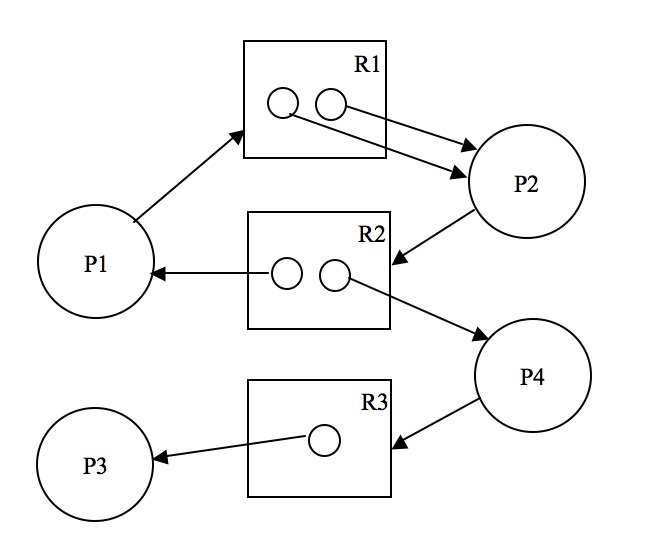
\includegraphics[scale=0.2]{res_alloc}
\end{center}

\section{Process synchronization}

The critical section problem could be solved simply by disallowing interrupts
on a single core cpu. With multiple cores, however, disabling these interrupts
will be too time consuming.

\subsection{Dekker's Algorithm}
Dekker's algorithm solves the process synchronization problem with busy waits.
Meaning: using the below specified code results in a correctl handling of
critical areas. Alas, the threads spend CPU cycles in the while loop, needlessly.
If we implement Dekker's we should compliment it with wait/notify functionality.
Without this improvement the semaphores can be referred to as spinlocks.
The only advantage with using spinlocks is that there is no context switch
required.

\begin{lstlisting}[label=dekkers,caption=Dekker's Algorithm]
public class Dekkers extends MutualExclusion {
  public Dekkers () {
    flag[0] = false;
    flag[1] = false;
    turn = TURN_0;
  }

  public void enteringCriticalSection (int t) {
    int other;

    other = 1 - t;

    flag[t] = true;
    turn = other;

    while ((flag[other] == true) && (turn == other)) {
      Thread.yield();
    }
  }

  public void leavingCriticalSection (int t) {
    flag[t] = false;
  }

  private volatile int turn;
  private volatile boolean[] flag = new boolean[2];
}
\end{lstlisting}

\subsection{Race condition}
A race condition is when multiple threads access and manipulate the same
data concurrently, and where outcome of the execution depends on the
particular order in which access takes place.

\subsection{Mutual Exclustion}
If thread $T_i$ is executing in its critical section, then no other threads
can be executing in their critical sections.

\subsection{Progress}
If no thread is executing in its critical section and there exist threads
that wish to enter their critical sections, then only the threads not executing
in their critical section get to partake in the process of deciding which
thread gets to execute its critical section next.

\subsection{Starvation}
When some threads are allowed to execute and make progress, but others are
left ``starving.''

\subsection{Livelock}
No thread makes progress, but they keep executing.

\subsection{Bounded waiting}
There exists a limit to the amount of times a thread will wait for other
threads before its request to enter a critical area is granted. (This
prevents starvation in a single thread.)

\subsection{Drifting}
The following piece of code will cause accumulative drift.
\begin{lstlisting}[label=drift,caption=Drift example]
while (!isInterrupted()) {
              sleep(100); foo.bar();
}
\end{lstlisting}

Sleep specifies a minimun time to sleep, and a context switch may have ocurred
after sleep and before the method call thus drift is accumulated.

\begin{lstlisting}[label=drift-fix,caption=Drift fixed]
long t = System.currentTimeMillis();
while (!isInterrupted()) {
  foo.bar();
  t += 100;
  long diff = t - System.currentTimeMillis();
  if (diff > 0) sleep(diff);
}
\end{lstlisting}

Even with this fix, sleep still causes a minimum busy wait.

\subsection{volatile, transient keywords}
Volatile means that the compiler is not allowed to cache the value of this
variable. It should be updated before evaluation.

Transient means that the variable has no meaning outside of its current context
if the variable is passed along with a serialized object over a network, it
gets set to ``null'' or its equivalence.

\section{Scheduling}
\subsection{Scheduler}
The scheduler schedules different threads for execution time on the CPU. As
explained above, there are three different states for the threads/processes:

\begin{itemize}
  \item \emph{Running:} the thread is executing its instructions on the CPU.
        The scheduler could decide that the thread has had enough execution time
        and move the thread \emph{from} running \emph{to} ready.
  \item \emph{Ready:} The thread has told the scheduler that it is ready for
        execution on the CPU. When the scheduler decides that the thread should
        get to execute, it initiates a context switch and transfers it into
        the running state.
  \item \emph{Blocked:} the thread has reached a point in its execution where
        it decides to yield the processor. This could be due to not being able
        to lock a resource or having to sleep. Important to note is that it is
        the thread itself that decides when to block. When the thread can continue
        it is usually due to another thread changing the state of something.
        It can thus be argued that it is the other thread that takes the first
        thread from blocked to ready.
\end{itemize}

\subsection{Context switch}
A context switch occurs for instance when the scheduler decides that the
current thread has run long enough, and allows another thread to execute. The
threads each have a call stack. This call stack together with the current
registers are saved away and the other thread's call stack and registers are
restored.

\subsubsection{Faster context switches}
Without preemption we can speed up the process of a context switch, since
we will then know exactly what needs to get saved away. With preemption we
cannot be entirely sure. Ergo we will need to save everything.

\subsection{Priority inversion phenomenon}
Occurs when a low priority thread manages to lock a resource and this thread
is then interrupted by a higher priority thread. When the thread requests the
same resource, the lower thread blocks the higher thread and can thus resume
its execution. (Despite being lower prioritized than the other thread.)
If we called the highest prioritized thead A, and call the lowest Z. If Z
blocks A, and Z is interrupted by a higher prioritized thread (M?) that doesn't
share its resources, then this thread (M) also blocks A. This is called a 
\emph{prioriy inversion} since Z and M will execute before A.

\subsection{Priority inheritence protocol}
The basic idea is to modify the priority of the tasks causing the blocking. In
particular when Z blocks higher prioritized tasks, it temporarily inherits the
highest priority of the blocked tasks. This prevents medium prioritized threads
from preempting Z and prolonging the blocking duration.
\subsubsection{Basic}
Raises the priority of the low priority thread temporarily
\subsubsection{Priority Ceiling Protocol}
To bound the priority inversion phenomenon and preent the formation of deadlocks
and chained blocking; PCP extends the priority inheritence protocol with a
rule for granting a lock request.

When a job enters a critical section it receives the \emph{priority ceiling} 
equal to the highest prioritized job able to access said resource, meaning that
once it enters the critical region. This means that the only time it is
interrupted is when a job with higher priority needs to run. (The interrupting
job doesn't access the lower prioritized job's resource.)

If a job with higher priority than the currently running job in the semaphore
tries to gain access, its priority is transferred to the lower prioritized job
ensuring that a job won't be interrupted again by some job of said priority or
lower.

\begin{enumerate}
  \item Each semaphore is assigned a priority ceiling equal to the highest
        priority of jobs that can lock it.
  \item The job with the highest priority gets to run first.
  \item The job running locks a semaphore.
  \item Another job tries to interrupt the currently running job, but if said
        job has a lower priority than the priority ceiling, the first job
        continues to run. If the interrupting job had a higher priority than
        the job running inside the semaphore, its priority is transferred to the
        currently running job. (Priority inheritence)
  \item When no others jobs are blocked by the thread it resumes its original
        priority, i.e. its ``nominal priority.''
  \item Priority inheritence is transitive. I.e. if job $J_3$ blocks $J_2$ which
        in turn blocks $J_1$ then $J_3$ may inherit the priority from $J_1$.
\end{enumerate}

\emph{Ceiling blocking} occurs when the highest prioritized task that can access
a resource is blocked by a lower prioritized job using the resource.

\subsubsection{Immediate inheritence}
The priority of the thread running in a semaphore is immediately raised to the
ceiling priority.

\subsection{Direct blocking}
Occurs when a higher-priority job tries to acquire resources held by a job
with lower priority.

\subsection{Push-through blocking}
Occurs when a medium priority job is blocked by a lower priority job that has
inherited a higher priority from a job it directly blocks. This is necessary
to avoid unbounded priority inversion.

\subsection{Rate monotonic scheduling}
Scheduling by rate of occurrence. I.e. a job that has a high occurrence rate is
highly prioritized. A set of tasks is said to be schedulable by the rate monotonic 
algorithm if 
\begin{center}
  $\sum_{i=1}^{n} \frac{C_i}{T_i} \leq n(2^{1/n}-1)$
\end{center}

The tasks are also schedulable if $R_i \leq C_i$ for all jobs. We define $R_i$ as:

\begin{center}
  $R_i = C_i + B_i + \sum_{j=1}^{i-1} \ceil{\frac{R_i}{T_j}}C_j$
\end{center}

\subsection{Chained blocking}
When a highly prioritized job needs to collect resources held by two or more
lower prioritized jobs, meaning it has to wait for a series of lower prioritized
jobs to finish before managing to complete its own tasks.

\section{Sceduling Theory}
\subsection{Sufficient and necessary}
The analysis is \emph{sufficient} if, when it answers ``YES'', all deadlines
are met.

The analysis is \emph{necesary} if, when it answers ``NO'', there reallys is a
situation where deadlines could be missed.

The analysis is \emph{exact} if it is both necessary and sufficient.

\subsection{Fixed priority scheduling}
With fixed priority scheduling, where to execute each task is decided
dynamically based on which of the currently ready tasks has the highest
priority.

\subsection{Execution time estimation}

\subsubsection{Measuring execution times}
The main problem with this approach is that it can be overly optimistic.
There are no guarantees that the longest execution time has occurred.
Testing all combinations of input data is often impossible in practice.
Caching and pipelining further exacerbate the estimations, the remedy to this
is typically to disable caching and pipelining.

\subsubsection{Analyzing execution times}
The main problem with the approach is that it can be overly pessimistic, however,
this approach  is the only one that is formally correct.

\begin{itemize}
  \item \emph{Compiler dependence:} different compilers generate different code
        typically analysis tools work with machine code.
  \item \emph{Data dependant branching:} analysis tool must explore all paths
        and return the longest.
  \item \emph{Iterations and recursion:} the programmer must specify the number
        of times a loop may execute. Also hard to know how deep recursion will
        go. Therefore it is often disallowed.
  \item \emph{Dynamic memory allocation:} may invoke garbage collection, which
        is extremely difficult for analysis tools to handle.
\end{itemize}

The gap between general purpose hardware and hardware which safely can be used
for hard real-time applications i.e. that can be analyzed increases. This makes
it important to develop theory and methods that make it possible to use general
purpose platforms in hard real-time applications with an acceptable level of
performance and quality of service.

\subsection{Scheduling methods}
\subsubsection{Static cyclic scheduling}
Static cyclic scheduling is an off-line approach. Contains a table of the order
in which to execute the different tasks. The table repeats cyclically.

The scheduler simply starts the first task in the calendar (table), awaits its
completion, waits until it's time to start the next task, waits for its
completion, and so on. The reason it cannoot start executing the second one
immediately is that the schedule has been calculated based on worst running
times. Making this rather ineffective but safe. In a slightly more complicated
case of preemptive scheduling, the schedule also contains how long each task is
allowed to run for.

Limitations:
\begin{itemize}
  \item \emph{Only periodic tasks:} aperiodic tasks are converted into periodic
        ones using polling.
  \item \emph{Long calendars:} The shortest repeating cycle is equal to the least
        common multiple between the task periods. For example: 5,10,20 ms gives
        the cycle 20 ms. But in this example: 7,13,23 ms the cycles length is
        2093 ms (least common denominator: $7*13*23=2093$)
  \item \emph{NP-completeness:} generating a schedule is a NP-hard problem.
\end{itemize}

The advantages:
\begin{itemize}
  \item \emph{Simple analysis:} only requirement is to run through the calendar
        and check weather all tasks meet their deadlines.
  \item \emph{Data sharing:} the scheduling algorithm can make sure that there
        won't be a context switch between tasks sharing data.
  \item \emph{Precedence constraints:} Possible to handle precedence constraints.
        I.e. X should finish before another task Y is allowed to start.
\end{itemize}

\subsection{Earliest Deadline First (EDF) Scheduling}

Tasks are scheduled according to which task has the earliest deadline. The
approach is dynamic. It is often more intuitive to assign deadlines to tasks
than it is to assign priorities. Assigning deadlines only requires local knowledge
whereas priorities require a complete understanding, i.e. global knowledge.

\begin{itemize}
  \item Only periodic tasks
  \item each task $i$ has a period of $T_i$
  \item required computation time $C_i$ (worst case)
  \item deadline $D_i = T_i$
  \item no interprocess communication
  \item an ``ideal'' real-time kernel
\end{itemize}

An \emph{ideal kernel} means that context switches and interrupts take zero time.
If the \emph{utilization} $U$ is less than $100\%$ then all deadlines will be met:

\begin{center}
$U = \sum_{i=1}^{i=n} \frac{C_i}{T_i} \leq 1$
\end{center}

The main advantage of EDF is that the processor can be fully utilized and still
all deadlines will be met.

\subsection{Rate monotonic scheduling}

Priorities are set monotonically according to task rate (period). A task with
shorter period is assigned a higher priority.

\begin{itemize}
  \item Only periodic tasks
  \item $D_i = T_i$
  \item $C_i$ are known
  \item No interprocess communication
  \item Tasks may not suspend themselves
  \item priorities are unique
  \item the kernel is ideal
\end{itemize}

With these assumptions, the following holds:

For a system with $n$ tasks, all tasks will meet their deadlines if:

\begin{center}
  $ \sum_{i=1}^{i=n} \frac{C_i}{T_i} \leq n(2^{1/n} - 1) $
\end{center}

The result is only sufficient. I.e. if the utilization is larger than the bound,
the task may still be schedulable. As $n \rightarrow \infty$, the utilization
bound $U \rightarrow 0.693$. Which has led to the simple rule of thumb saying
that if the utilization is less than $0.693$ all deadlines are met.

\subsubsection{Generalized RMS}
Restrictive assumptions have been relaxed, in the following way: $D_i \leq T_i$.
We can also assume that the worst possible response time will be $\leq T_i$.

Also for a system with utilization larger than $0.693$ all deadlines will still
be met if:

\begin{center}
  $\forall i, R_i \leq D_i$
\end{center}
where:
\begin{center}
  $R_i^{n+1} = C_i + B_i + \sum_{\forall j \in hp(i)} \ceil{\frac{R_i}{T_j}} C_j, R_i^0 = 0$
\end{center}

Stated earlier RMS didn't take interprocess communication into account. The above,
however, includes $B_i$ i.e. blocking time. Thus RMS can be expanded to cover
interprocess communication (and release jitter, but fuck that).

For RMS to work all $C_i$ have to be known. Something which is extremely difficult.
Worst-case execution times are much larger than those that occur in practice.
Thus many cases may be considered to be unschedulable but will work perfectly fine
in reality.

Another form of measurement for schedulability using RMS is the \emph{hyperbolic bound}
which recently proved that a task is schedulable if:

\begin{center}
  $\prod_{i=1}^{n} U_i + 1 \leq 2$, where $U_i = \frac{C_i}{T_i}$
\end{center}


\subsubsection{Calculating $B_i$}
In RMS a thread can only be blocked by a \emph{lower} priority thread. Remember that
it can thus be blocked by push-through blocking.

\begin{enumerate}
  \item The monitor to which the thread is connected, which of the lower
        priority threads can block it? Calculate max of these.
  \item Can it be blocked on a different monitor? The value from 1 added to this.
  \item Can it be blocked by push-through blocking? Take this into account.
\end{enumerate}

\subsubsection{Calculating $C_i$}
If $R_i$ or $T_i$ and $B_i$ is known we may calculate the smallest possible $C_i$
using the following chain of reasoning: \\

\emph{Example:} $R_i = 50$,$B_i = 10$ and i has one higher priority thread,
A, with $T_A = 100$ and $C_A = 10$. This gives us:
\begin{center}
  $R_i = C_i + B_i + \sum_{\forall k \in hp(k)} \ceil{\frac{R_k}{T_j}} C_j = 50$ \\
  $\Longleftrightarrow$ \\
  $90 = C_i + 10 + \ceil{\frac{90}{100}} 10$ \\
  $C_i = 70$
\end{center}

\section{Garbage collection}

\subsection{Manual memory management}
Using manual memory management we have to make sure that we get no dangling
pointers and no memory leaks. Even if we do this, we can't be sure that the
heap is properly defragmented. (GC without compaction also leads to this.)

\subsection{Reference Counting}
We keep a count to how many references a certain object in memory has. When
this counter reaches zero we remove the object.

\emph{Advantages:} Easy to implement, short pauses.
\emph{Disadvantages:} 
\begin{itemize}
  \item DEqueues will have circular references, meaning they won't
        be marked for removal by the GC.
  \item No compaction $\rightarrow$ fragmentation
  \item Expensive, the counters have to be adjusted for every pointer
        assignment.
\end{itemize}
\subsection{Traversing algorithms}
The idea is to periodically traverse the objects in the heap from a root
pointer, usually located in or near main. Objects that are encountered
are marked, and the ones not marked are deleted.

\subsubsection{Cheney's algorithm}
The heap is divided into two equal halves, only one of which is in use at any
one time. Garbage collection is performed by copying live objects from one heap
to the next, which then becomes current heap. The entire old heap can then be
discarded in one piece.

A pointer from the old object location to the new one is kept during copy so
that the program can still run during garbage collection.

\subsubsection{Generation-based GC}
It stands to reason that if objects die young, the ones that don't usually
live for a long time.

\begin{itemize}
  \item Partition heap into several generations
  \item New objects are allocated into the young generation
  \item Surviving objects are promoted into the next generation
\end{itemize}

\emph{Pros:} Efficient! Most pauses are short. Most garbage collection is done
             in the youngest generation.
\emph{Cons:} Complex. Must keep track of inter-generation pointers.

\subsubsection{Idea}
By our own Roger Henriksson!
\begin{itemize}
  \item Avoid doing GC work when high-priority threads execute.
  \item Perform GC in the pauses. Memory always available.
  \item Low-priority threads: standard incremental techniques.
  \item Minimize the cost for pointer operations for the high-
        priority threads.
  \item Interruptible garbage collection, minimum locking.
  \item Theory for a priori schedulability analysis.
\end{itemize}

\subsection{Implementation details}
For the garbage collector not getting in the way of things, with a similar
scenario, the following should be done:

\begin{itemize}
  \item Assuming we have one HP thread and one LP thread.
  \item Garbage collection should be scheduled after the HP thread has run.
        I.e. the GC should have a medium priority.
  \item Cleaning after the LP thread should be done in its context. I.e. the
        GC should have the same priority as the LP for cleaning up after said
        thread.
\end{itemize}






\end{document}
